\chapter{Programming}\label{chap:programming}
This project required over $450$ labelings of various forests, all of which were found by hand. At around $200$ labelings it became clear that due to the sheer number of labelings being done, just probablistically some labelings would (1) have typos (2) have incorrect computations and (3) violate some constraint of the labeling.

All this programming began because we wanted some sort of local program that could display the labelings, so we could check with some level of certainty that they were isomorphic to the forest being worked with. Everything we found that displayed graphs didn't allow for dragging vertices and/or interacting with graphs at a high level. So we decided to make our own programs.

There are three groups of programs in a dedicated github repository that we provide links to, for the sake of space. Note: the dependencies required to run these are:

\setlist[enumerate,1]{label=(\arabic*)}
\begin{enumerate}
  \item A \verb|python| 3.13 installation
  \item The \verb|NetworkX| library for \verb|python|
  \item the \verb|pygame| or \verb|pygame-ce| library for \verb|python|
  \item the \verb|itertools| library for \verb|python|
  \item the \verb|z3| library for \verb|python|
\end{enumerate}
It should be clear when looking at the code what the dependencies are. If you use \verb|pip| in \verb|vscode|, you may simply input the following into your workspace terminal: 
\begin{verbatim}
py -m pip install #enter library name here
# OR
python -m pip install #enter library name here
\end{verbatim}
depending on how you install and work with \verb|python|, installing packages may not work this way. \verb|Anaconda| is a popular \verb|python| bundle that likely comes with some of these.

\section{Tikzgrapher}

The file shared here is an earlier version of a program named \verb|tikzgrapher| that was specifically built to display (1-2-3)-labelings and 1-rotational (1-2-3)-labelings. There is a less restrictive version where arguments are optional and customizable (custom edge and vertex labelings, colorings of vertices, no side tab for squares containing lengths). Here is a link to the newer version of \verb|tikzgrapher|: $\newline$\url{https://github.com/tucxy/Programming/tree/main/Python/tikzgrapher}

These are the features ordered earliest to latest in this older build of \verb|tikzgrapher|:
\setlist[enumerate,1]{label=(\arabic*)}
\begin{enumerate}
  \item Displays a list of \verb|NetworkX| graphs together on one \verb|pygame| window, starting from top to bottom.
  \item Reduces vertices modulo $n$ and computes the standard edge length for each edge modulo $n$, and has the subscript as the additive edge length $\ell_{7}^{+}$.
  \item For each graph in the list given as input: uses a longest path search algorithm and by default displays the longest path of a graph in the center row of a grid of coordinates, then displays vertices coming off of that row.
  \item Has a tab on the left that displays all standard edge lengths $\ell$ and a chart for the subscript labels of the labelings in order. The window with the tab open looks similar to Figure \ref{fig:K21labelingex} except it doesn't have colored edges.
  \item Allows user to save displayed graphs as a \verb|Tikz| graph in a standalone \LaTeX$\,$file to a specified path.
\end{enumerate}
We have every single forest labeling in files that import this version \verb|tikzgrapher|. If you simply uncomment below a forest, a \verb|pygame| window will pop out and display the labeling. Here are links to those files.
\begin{enumerate}
  \item $\sigma^{+-}$-labelings: $\newline$\url{https://github.com/tucxy/Thesis-Programs/blob/main/sigma.py}
  \item (1-2-3)-labelings: $\newline$\url{https://github.com/tucxy/Thesis-Programs/blob/main/7mod14.py}
  \item 1-rotational (1-2-3)-labelings: $\newline$\url{https://github.com/tucxy/Thesis-Programs/blob/main/8mod14.py}
  \item $\mathbf{T_{7}^{11}\sqcup T_{2}^{1}}$-decomposition of $K_{21}$ and $K_{22}$: $\newline$\url{https://github.com/tucxy/Thesis-Programs/blob/main/starpath.py}
\end{enumerate}


\begin{figure}[H]
  \centering
  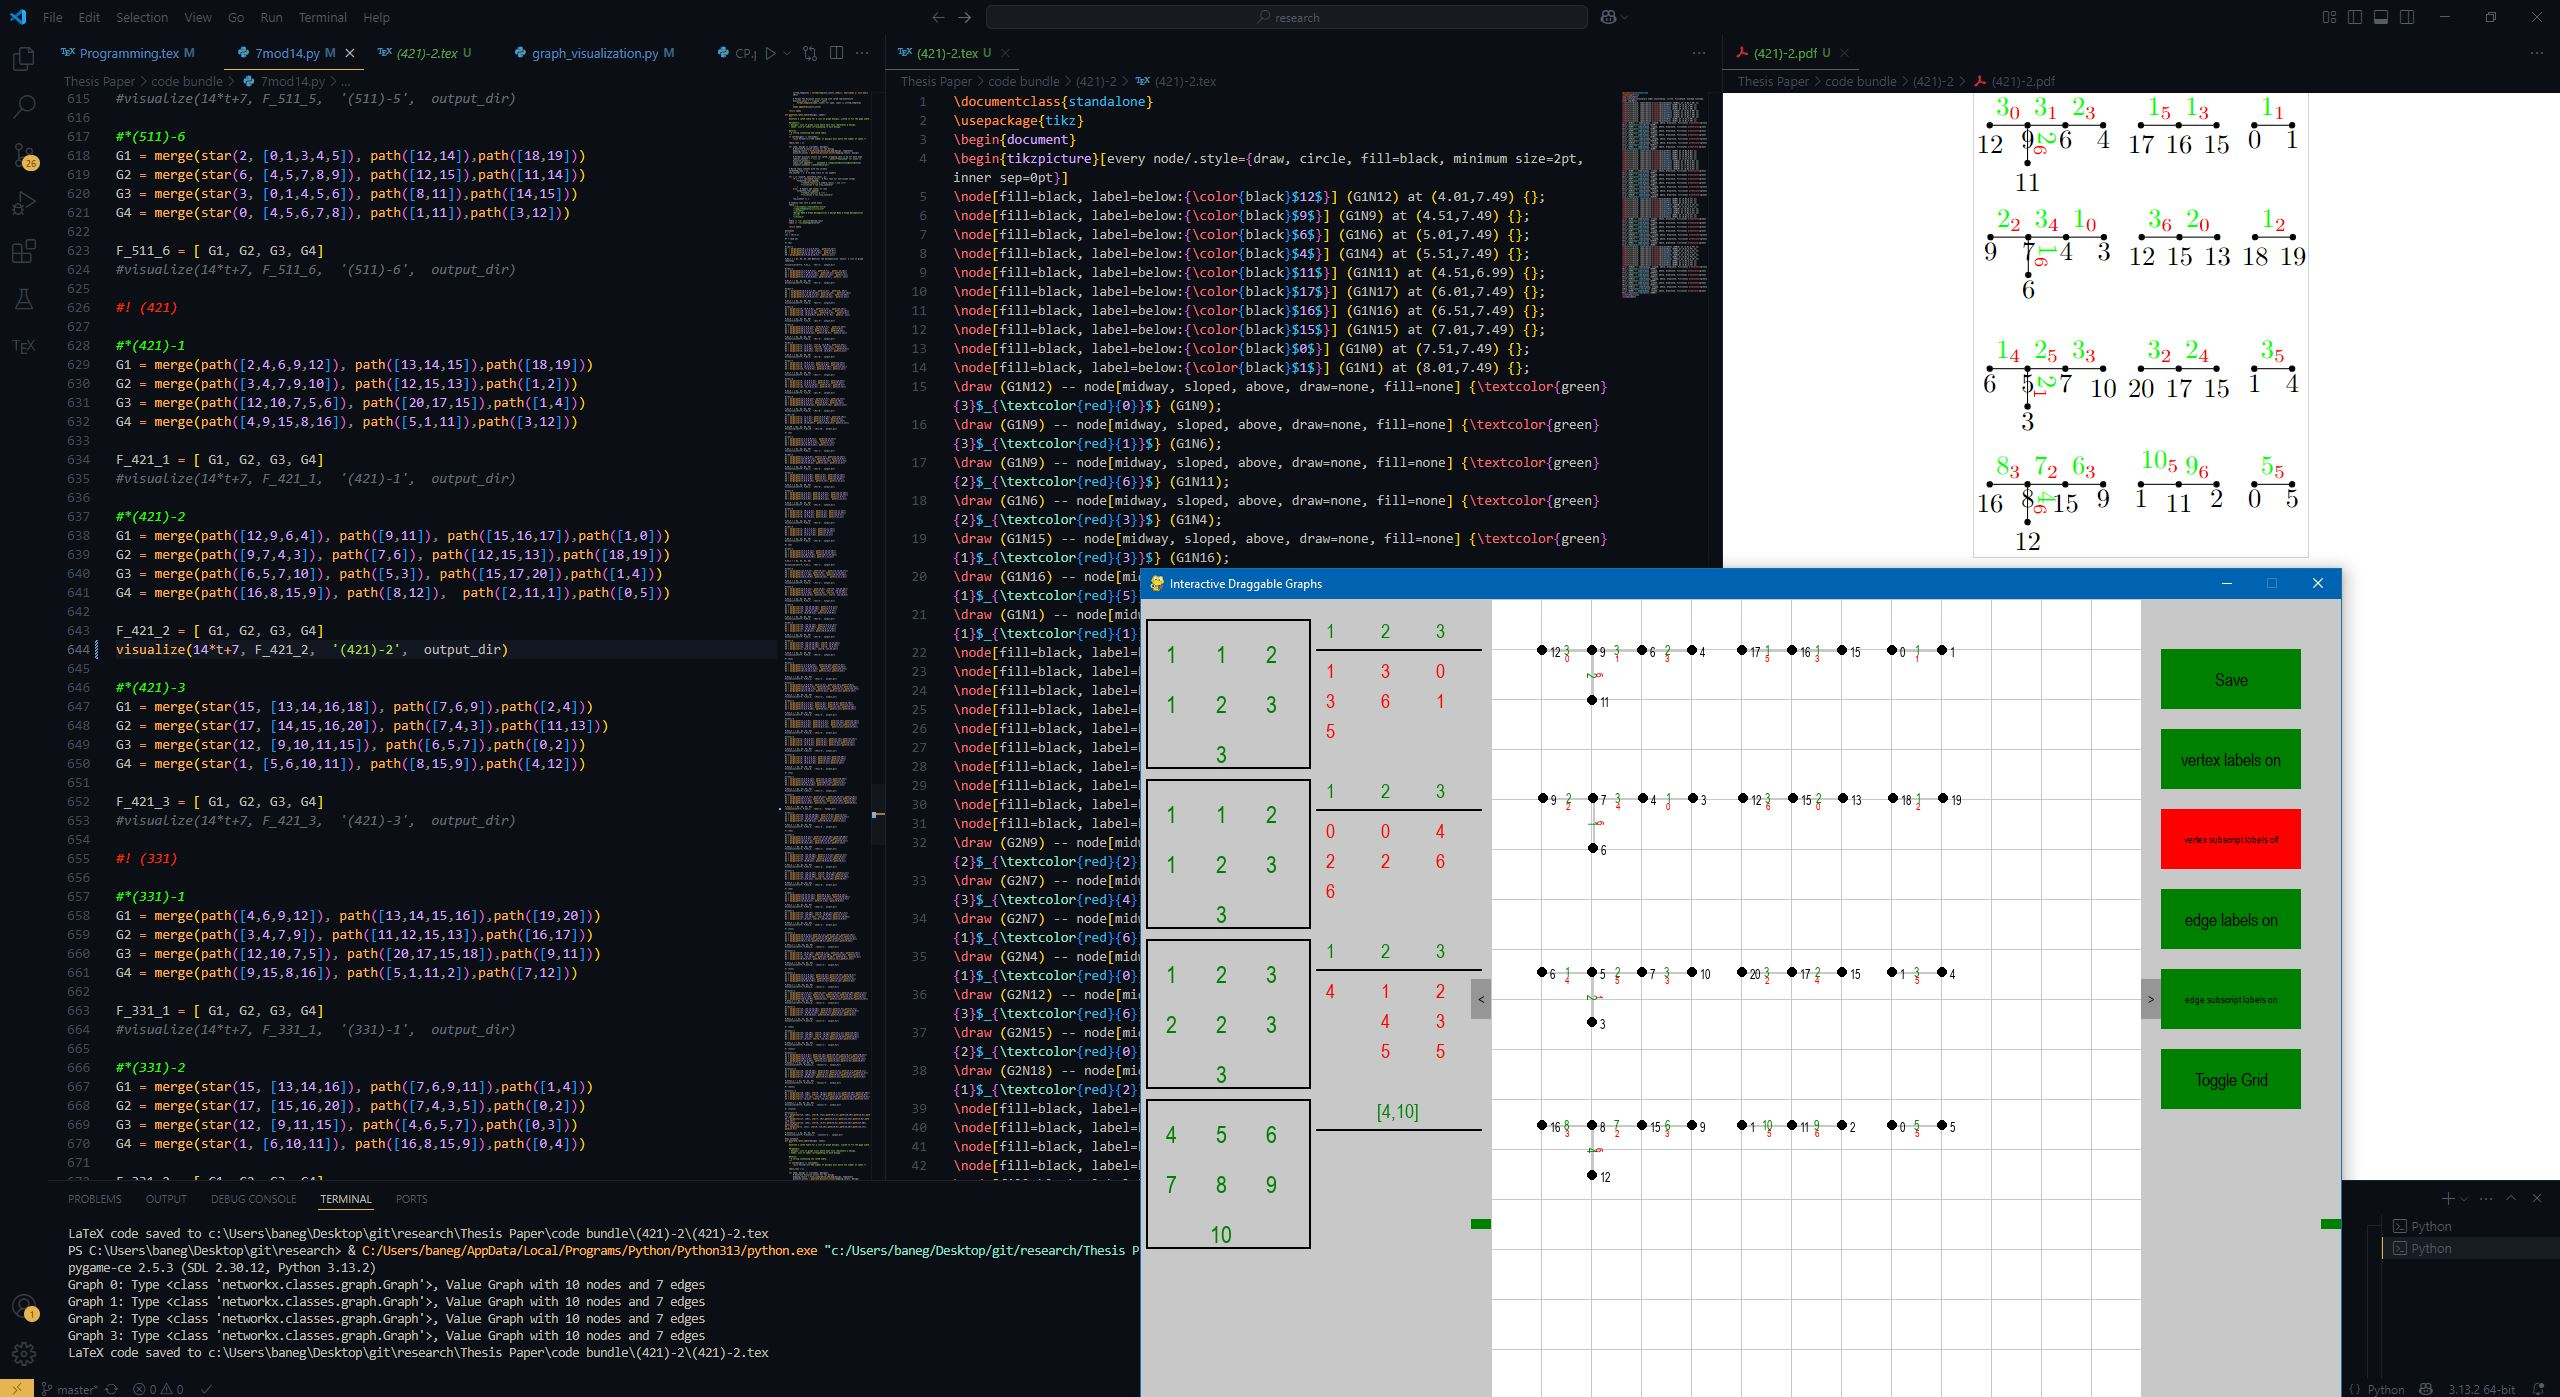
\includegraphics[width=\textwidth]{standalone/Images/snippet_long.JPG}
  \caption{A snippet of \textit{tikzgrapher}}
  \label{fig:TGsnippet}
\end{figure}


Once again, this version is no longer being updated, the following link will take you to the latest version: $\newline$\url{https://github.com/tucxy/Programming/tree/main/Python/tikzgrapher} \newline

\section{Labeling Solvers}
This next program is a bit more ambitious. After all labelings were found (of course) we thought, "Hey what if we didn't have to find these by hand?" Initially, we tried to use a genetic learning algorithm but found that the fitness function was too rigid, and realized that reinforcement learning was not the way to go. We found much more success using constraint programming. Using the \verb|z3| SAT solver, we created (1) a solver that outputs a $\sigma^{+-}$-labeling of a graph (2) a graceful labeling of a graph (3) a solver that oututs a more generalized version of the (1-2-3)-labeling for a graph on $m$ edges in $K_{2mt+r}$ where $r$ is an odd idempotent modulo $2m$.

The $\sigma^{+-}$-labeling is quite fast, but the other labelings can take up to five minutes or so. In the future, we hope to translate this code to \verb|C++|, to hopefully speed up the process. As of now, it does work and the beefier the processor the better. Here are the links to this project:

\begin{enumerate}
  \item  Labeling Solvers: $\newline$\url{https://github.com/tucxy/Thesis-Programs/blob/main/CP.py}
  \item  Notebook to test the solvers: $\newline$\url{https://github.com/tucxy/Thesis-Programs/blob/main/main.py}
\end{enumerate}

\begin{figure}[H]
  \begin{center}
  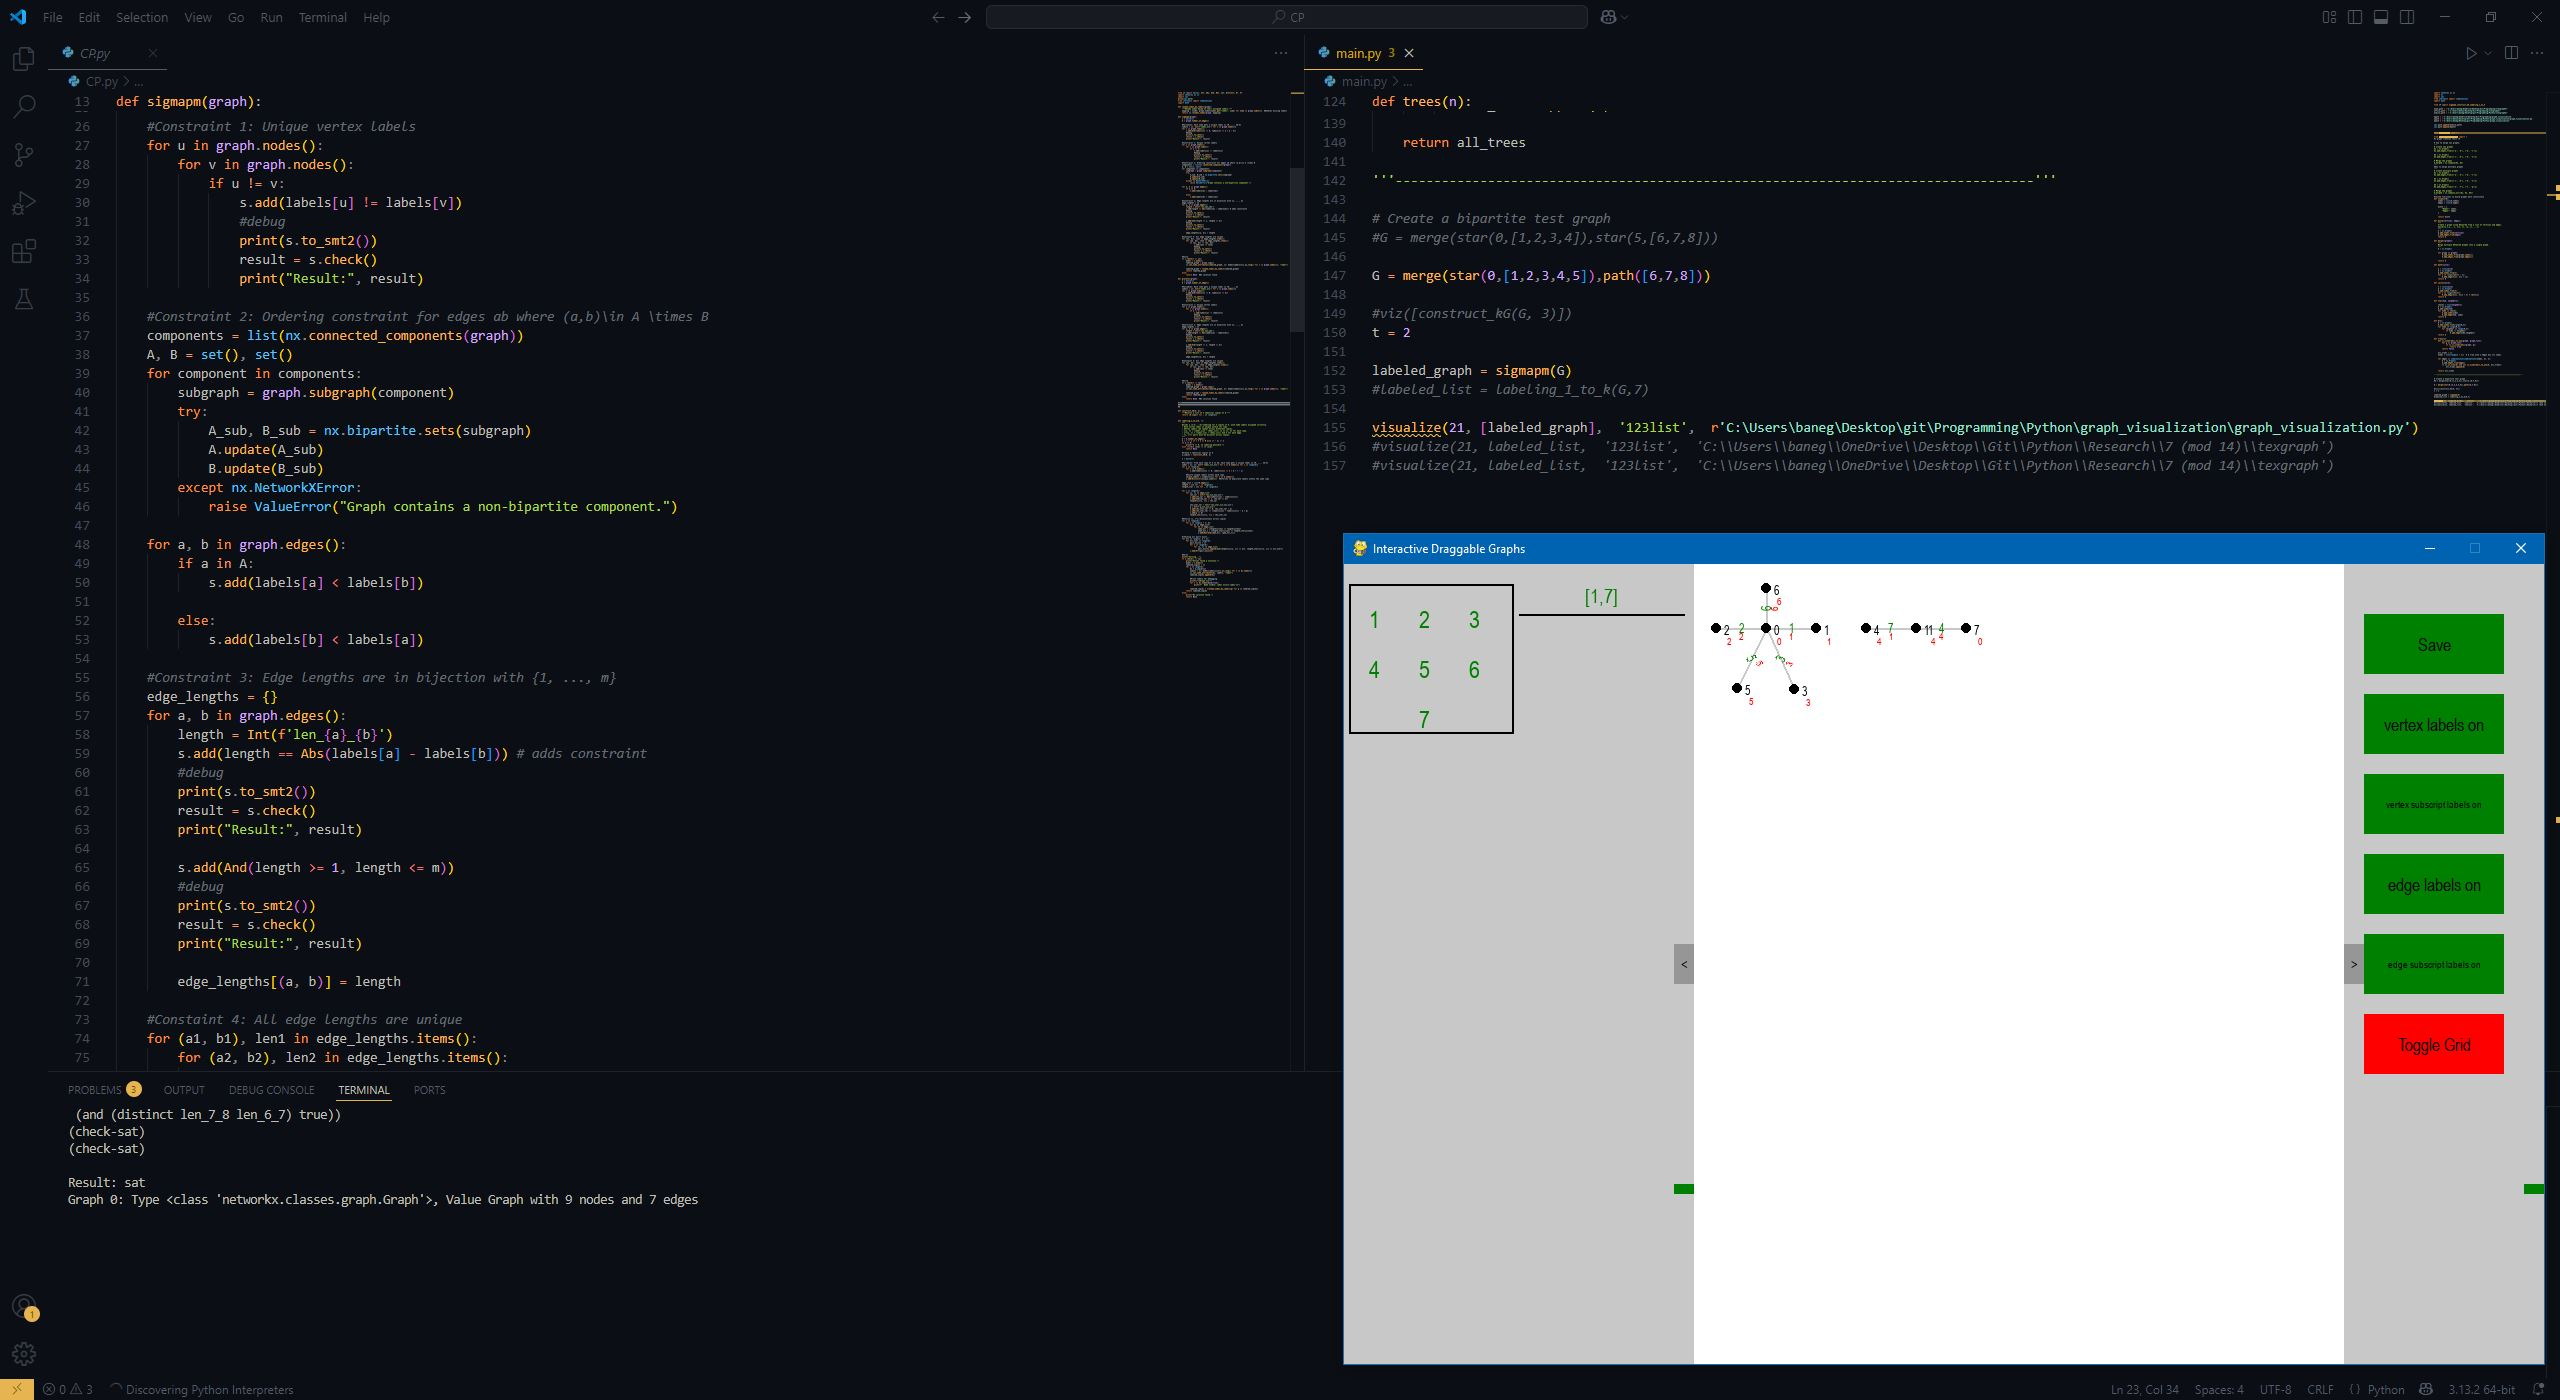
\includegraphics[width=0.8\textwidth]{standalone/Images/CPsnippetlong.JPG}
  \caption{A snippet of the $\sigma^{+-}$-labeling solver}
  \label{fig:CPsnippet}
  \end{center}
\end{figure}


These are set up so that if you visit this link: $\newline$\url{https://github.com/tucxy/Thesis-Programs/tree/main} and click the code button: the .zip file installed will give a folder when extracted. Make that folder your working directory, and everything should just work.

\begin{figure}[H]
  \begin{center}
  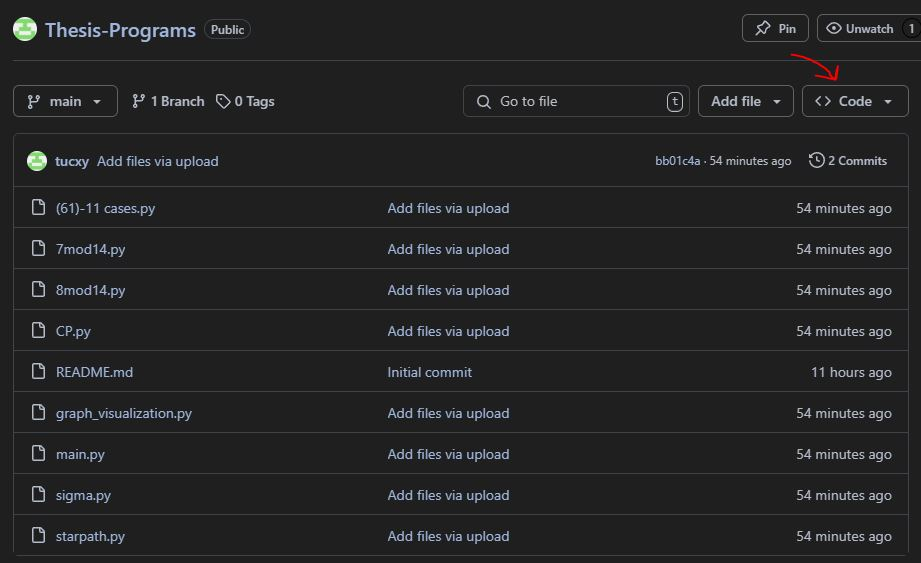
\includegraphics[width=0.8\textwidth]{standalone/Images/guide.JPG}
  \caption{click on the code button to download the zip file. Then extract the folder and set it as your working directory.}
  \label{fig:CPsnippet}
  \end{center}
\end{figure}

Feel free to email me with questions: baneg003@outlook.com